% Created by tikzDevice version 0.12.3.1 on 2021-06-16 15:27:58
% !TEX encoding = UTF-8 Unicode
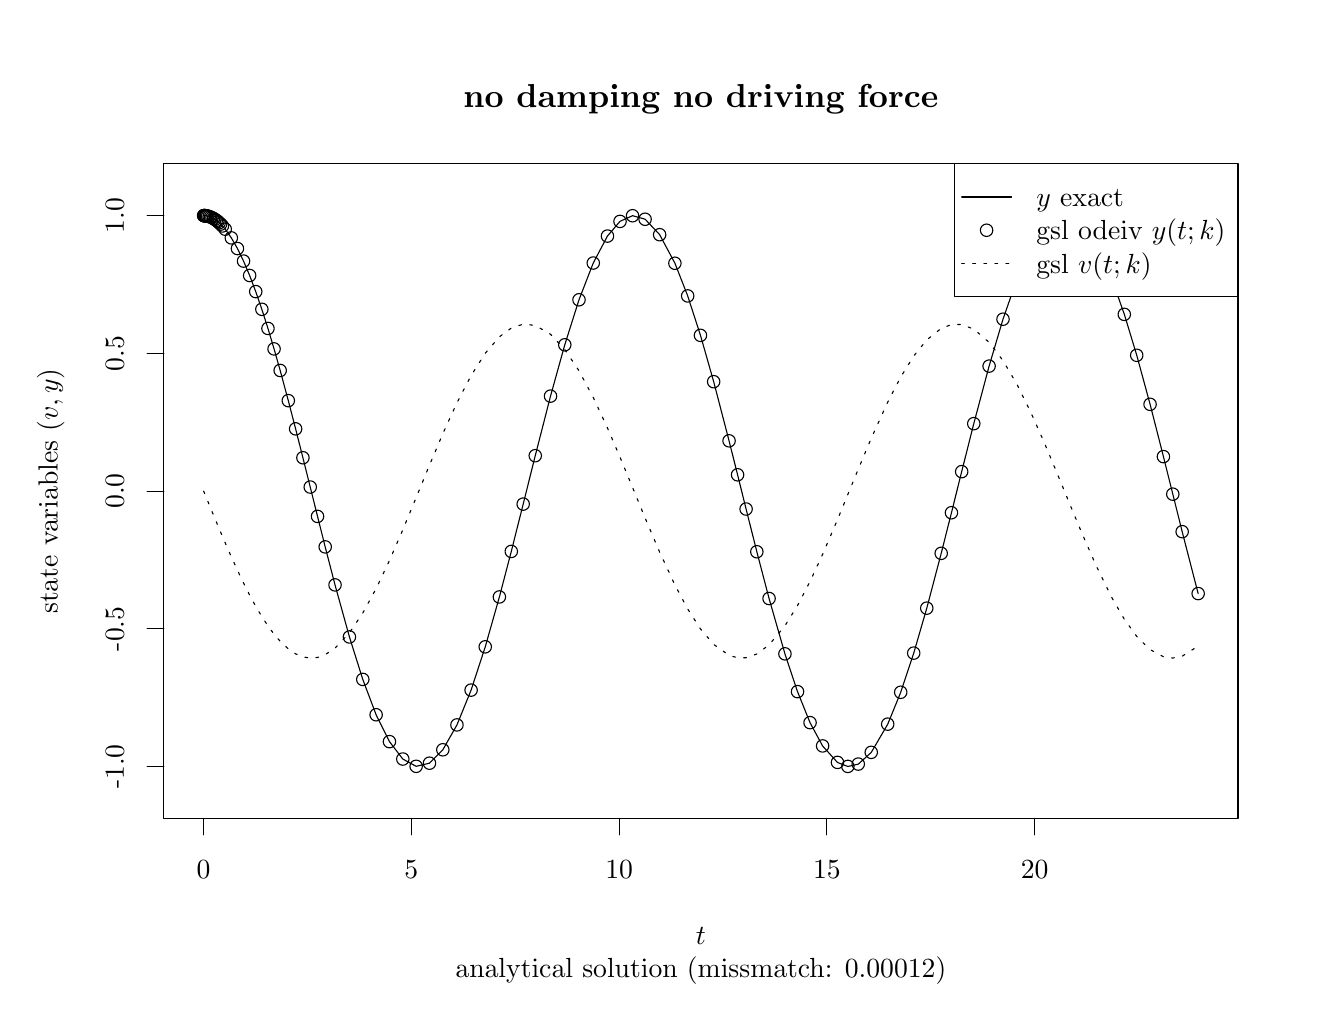
\begin{tikzpicture}[x=1pt,y=1pt]
\definecolor{fillColor}{RGB}{255,255,255}
\path[use as bounding box,fill=fillColor,fill opacity=0.00] (0,0) rectangle (462.53,346.90);
\begin{scope}
\path[clip] ( 49.20, 61.20) rectangle (437.33,297.70);
\definecolor{drawColor}{RGB}{0,0,0}

\path[draw=drawColor,line width= 0.4pt,line join=round,line cap=round] ( 63.58,278.98) --
	( 63.66,278.98) --
	( 63.76,278.98) --
	( 63.86,278.98) --
	( 63.97,278.97) --
	( 64.07,278.96) --
	( 64.18,278.95) --
	( 64.28,278.94) --
	( 64.43,278.92) --
	( 64.66,278.89) --
	( 65.06,278.81) --
	( 65.57,278.66) --
	( 66.09,278.47) --
	( 66.61,278.23) --
	( 67.13,277.96) --
	( 67.65,277.64) --
	( 68.17,277.27) --
	( 68.69,276.87) --
	( 69.21,276.42) --
	( 69.73,275.92) --
	( 70.38,275.24) --
	( 71.38,274.08) --
	( 73.59,270.95) --
	( 75.80,267.10) --
	( 78.00,262.55) --
	( 80.21,257.34) --
	( 82.41,251.52) --
	( 84.62,245.12) --
	( 86.83,238.20) --
	( 89.03,230.82) --
	( 91.24,223.03) --
	( 94.18,212.12) --
	( 96.82,201.93) --
	( 99.46,191.48) --
	(102.10,180.90) --
	(104.74,170.29) --
	(107.51,159.27) --
	(111.06,145.54) --
	(116.27,126.73) --
	(121.09,111.39) --
	(125.91, 98.62) --
	(130.73, 88.91) --
	(135.55, 82.62) --
	(140.37, 79.99) --
	(145.19, 81.12) --
	(150.01, 85.96) --
	(155.12, 94.95) --
	(160.23,107.53) --
	(165.34,123.16) --
	(170.45,141.18) --
	(174.75,157.63) --
	(179.05,174.74) --
	(183.41,192.23) --
	(188.93,213.76) --
	(194.08,232.30) --
	(199.22,248.57) --
	(204.37,261.86) --
	(209.51,271.61) --
	(214.04,276.91) --
	(218.57,278.96) --
	(223.10,277.69) --
	(228.36,272.11) --
	(233.87,261.80) --
	(238.49,249.99) --
	(243.11,235.74) --
	(247.88,218.99) --
	(253.44,197.62) --
	(256.52,185.34) --
	(259.60,172.97) --
	(263.48,157.52) --
	(267.90,140.63) --
	(273.64,120.62) --
	(278.18,106.97) --
	(282.71, 95.75) --
	(287.25, 87.34) --
	(292.62, 81.38) --
	(296.37, 79.93) --
	(300.13, 80.77) --
	(304.82, 85.01) --
	(310.77, 95.19) --
	(315.47,106.72) --
	(320.17,120.86) --
	(324.88,137.11) --
	(330.10,156.93) --
	(333.80,171.60) --
	(337.50,186.46) --
	(341.87,203.80) --
	(347.41,224.61) --
	(352.43,241.56) --
	(357.46,255.97) --
	(362.48,267.23) --
	(367.51,274.89) --
	(371.90,278.38) --
	(376.30,278.76) --
	(380.79,275.92) --
	(386.20,268.31) --
	(391.77,256.06) --
	(396.26,243.35) --
	(400.75,228.55) --
	(405.57,210.84) --
	(410.40,191.93) --
	(413.79,178.35) --
	(417.17,164.79) --
	(422.95,142.41);
\end{scope}
\begin{scope}
\path[clip] (  0.00,  0.00) rectangle (462.53,346.90);
\definecolor{drawColor}{RGB}{0,0,0}

\path[draw=drawColor,line width= 0.4pt,line join=round,line cap=round] ( 63.58, 61.20) -- (363.85, 61.20);

\path[draw=drawColor,line width= 0.4pt,line join=round,line cap=round] ( 63.58, 61.20) -- ( 63.58, 55.20);

\path[draw=drawColor,line width= 0.4pt,line join=round,line cap=round] (138.64, 61.20) -- (138.64, 55.20);

\path[draw=drawColor,line width= 0.4pt,line join=round,line cap=round] (213.71, 61.20) -- (213.71, 55.20);

\path[draw=drawColor,line width= 0.4pt,line join=round,line cap=round] (288.78, 61.20) -- (288.78, 55.20);

\path[draw=drawColor,line width= 0.4pt,line join=round,line cap=round] (363.85, 61.20) -- (363.85, 55.20);

\node[text=drawColor,anchor=base,inner sep=0pt, outer sep=0pt, scale=  1.00] at ( 63.58, 39.60) {0};

\node[text=drawColor,anchor=base,inner sep=0pt, outer sep=0pt, scale=  1.00] at (138.64, 39.60) {5};

\node[text=drawColor,anchor=base,inner sep=0pt, outer sep=0pt, scale=  1.00] at (213.71, 39.60) {10};

\node[text=drawColor,anchor=base,inner sep=0pt, outer sep=0pt, scale=  1.00] at (288.78, 39.60) {15};

\node[text=drawColor,anchor=base,inner sep=0pt, outer sep=0pt, scale=  1.00] at (363.85, 39.60) {20};

\path[draw=drawColor,line width= 0.4pt,line join=round,line cap=round] ( 49.20, 79.91) -- ( 49.20,278.98);

\path[draw=drawColor,line width= 0.4pt,line join=round,line cap=round] ( 49.20, 79.91) -- ( 43.20, 79.91);

\path[draw=drawColor,line width= 0.4pt,line join=round,line cap=round] ( 49.20,129.68) -- ( 43.20,129.68);

\path[draw=drawColor,line width= 0.4pt,line join=round,line cap=round] ( 49.20,179.45) -- ( 43.20,179.45);

\path[draw=drawColor,line width= 0.4pt,line join=round,line cap=round] ( 49.20,229.22) -- ( 43.20,229.22);

\path[draw=drawColor,line width= 0.4pt,line join=round,line cap=round] ( 49.20,278.98) -- ( 43.20,278.98);

\node[text=drawColor,rotate= 90.00,anchor=base,inner sep=0pt, outer sep=0pt, scale=  1.00] at ( 34.80, 79.91) {-1.0};

\node[text=drawColor,rotate= 90.00,anchor=base,inner sep=0pt, outer sep=0pt, scale=  1.00] at ( 34.80,129.68) {-0.5};

\node[text=drawColor,rotate= 90.00,anchor=base,inner sep=0pt, outer sep=0pt, scale=  1.00] at ( 34.80,179.45) {0.0};

\node[text=drawColor,rotate= 90.00,anchor=base,inner sep=0pt, outer sep=0pt, scale=  1.00] at ( 34.80,229.22) {0.5};

\node[text=drawColor,rotate= 90.00,anchor=base,inner sep=0pt, outer sep=0pt, scale=  1.00] at ( 34.80,278.98) {1.0};

\path[draw=drawColor,line width= 0.4pt,line join=round,line cap=round] ( 49.20, 61.20) --
	(437.33, 61.20) --
	(437.33,297.70) --
	( 49.20,297.70) --
	( 49.20, 61.20);
\end{scope}
\begin{scope}
\path[clip] (  0.00,  0.00) rectangle (462.53,346.90);
\definecolor{drawColor}{RGB}{0,0,0}

\node[text=drawColor,anchor=base,inner sep=0pt, outer sep=0pt, scale=  1.20] at (243.26,318.16) {\bfseries  no damping no driving force};

\node[text=drawColor,anchor=base,inner sep=0pt, outer sep=0pt, scale=  1.00] at (243.26,  3.60) {analytical solution (missmatch: 0.00012)};

\node[text=drawColor,anchor=base,inner sep=0pt, outer sep=0pt, scale=  1.00] at (243.26, 15.60) {$t$};

\node[text=drawColor,rotate= 90.00,anchor=base,inner sep=0pt, outer sep=0pt, scale=  1.00] at ( 10.80,179.45) {state variables $(v,y)$};
\end{scope}
\begin{scope}
\path[clip] ( 49.20, 61.20) rectangle (437.33,297.70);
\definecolor{drawColor}{RGB}{0,0,0}

\path[draw=drawColor,line width= 0.4pt,line join=round,line cap=round] ( 63.58,278.98) circle (  2.25);

\path[draw=drawColor,line width= 0.4pt,line join=round,line cap=round] ( 63.66,278.98) circle (  2.25);

\path[draw=drawColor,line width= 0.4pt,line join=round,line cap=round] ( 63.76,278.98) circle (  2.25);

\path[draw=drawColor,line width= 0.4pt,line join=round,line cap=round] ( 63.86,278.97) circle (  2.25);

\path[draw=drawColor,line width= 0.4pt,line join=round,line cap=round] ( 63.97,278.97) circle (  2.25);

\path[draw=drawColor,line width= 0.4pt,line join=round,line cap=round] ( 64.07,278.96) circle (  2.25);

\path[draw=drawColor,line width= 0.4pt,line join=round,line cap=round] ( 64.18,278.95) circle (  2.25);

\path[draw=drawColor,line width= 0.4pt,line join=round,line cap=round] ( 64.28,278.94) circle (  2.25);

\path[draw=drawColor,line width= 0.4pt,line join=round,line cap=round] ( 64.43,278.92) circle (  2.25);

\path[draw=drawColor,line width= 0.4pt,line join=round,line cap=round] ( 64.66,278.88) circle (  2.25);

\path[draw=drawColor,line width= 0.4pt,line join=round,line cap=round] ( 65.06,278.80) circle (  2.25);

\path[draw=drawColor,line width= 0.4pt,line join=round,line cap=round] ( 65.57,278.65) circle (  2.25);

\path[draw=drawColor,line width= 0.4pt,line join=round,line cap=round] ( 66.09,278.46) circle (  2.25);

\path[draw=drawColor,line width= 0.4pt,line join=round,line cap=round] ( 66.61,278.23) circle (  2.25);

\path[draw=drawColor,line width= 0.4pt,line join=round,line cap=round] ( 67.13,277.95) circle (  2.25);

\path[draw=drawColor,line width= 0.4pt,line join=round,line cap=round] ( 67.65,277.63) circle (  2.25);

\path[draw=drawColor,line width= 0.4pt,line join=round,line cap=round] ( 68.17,277.27) circle (  2.25);

\path[draw=drawColor,line width= 0.4pt,line join=round,line cap=round] ( 68.69,276.86) circle (  2.25);

\path[draw=drawColor,line width= 0.4pt,line join=round,line cap=round] ( 69.21,276.41) circle (  2.25);

\path[draw=drawColor,line width= 0.4pt,line join=round,line cap=round] ( 69.73,275.92) circle (  2.25);

\path[draw=drawColor,line width= 0.4pt,line join=round,line cap=round] ( 70.38,275.24) circle (  2.25);

\path[draw=drawColor,line width= 0.4pt,line join=round,line cap=round] ( 71.38,274.08) circle (  2.25);

\path[draw=drawColor,line width= 0.4pt,line join=round,line cap=round] ( 73.59,270.94) circle (  2.25);

\path[draw=drawColor,line width= 0.4pt,line join=round,line cap=round] ( 75.80,267.09) circle (  2.25);

\path[draw=drawColor,line width= 0.4pt,line join=round,line cap=round] ( 78.00,262.55) circle (  2.25);

\path[draw=drawColor,line width= 0.4pt,line join=round,line cap=round] ( 80.21,257.35) circle (  2.25);

\path[draw=drawColor,line width= 0.4pt,line join=round,line cap=round] ( 82.41,251.52) circle (  2.25);

\path[draw=drawColor,line width= 0.4pt,line join=round,line cap=round] ( 84.62,245.13) circle (  2.25);

\path[draw=drawColor,line width= 0.4pt,line join=round,line cap=round] ( 86.83,238.21) circle (  2.25);

\path[draw=drawColor,line width= 0.4pt,line join=round,line cap=round] ( 89.03,230.82) circle (  2.25);

\path[draw=drawColor,line width= 0.4pt,line join=round,line cap=round] ( 91.24,223.03) circle (  2.25);

\path[draw=drawColor,line width= 0.4pt,line join=round,line cap=round] ( 94.18,212.13) circle (  2.25);

\path[draw=drawColor,line width= 0.4pt,line join=round,line cap=round] ( 96.82,201.93) circle (  2.25);

\path[draw=drawColor,line width= 0.4pt,line join=round,line cap=round] ( 99.46,191.49) circle (  2.25);

\path[draw=drawColor,line width= 0.4pt,line join=round,line cap=round] (102.10,180.90) circle (  2.25);

\path[draw=drawColor,line width= 0.4pt,line join=round,line cap=round] (104.74,170.30) circle (  2.25);

\path[draw=drawColor,line width= 0.4pt,line join=round,line cap=round] (107.51,159.28) circle (  2.25);

\path[draw=drawColor,line width= 0.4pt,line join=round,line cap=round] (111.06,145.54) circle (  2.25);

\path[draw=drawColor,line width= 0.4pt,line join=round,line cap=round] (116.27,126.73) circle (  2.25);

\path[draw=drawColor,line width= 0.4pt,line join=round,line cap=round] (121.09,111.39) circle (  2.25);

\path[draw=drawColor,line width= 0.4pt,line join=round,line cap=round] (125.91, 98.62) circle (  2.25);

\path[draw=drawColor,line width= 0.4pt,line join=round,line cap=round] (130.73, 88.91) circle (  2.25);

\path[draw=drawColor,line width= 0.4pt,line join=round,line cap=round] (135.55, 82.62) circle (  2.25);

\path[draw=drawColor,line width= 0.4pt,line join=round,line cap=round] (140.37, 79.99) circle (  2.25);

\path[draw=drawColor,line width= 0.4pt,line join=round,line cap=round] (145.19, 81.12) circle (  2.25);

\path[draw=drawColor,line width= 0.4pt,line join=round,line cap=round] (150.01, 85.96) circle (  2.25);

\path[draw=drawColor,line width= 0.4pt,line join=round,line cap=round] (155.12, 94.95) circle (  2.25);

\path[draw=drawColor,line width= 0.4pt,line join=round,line cap=round] (160.23,107.53) circle (  2.25);

\path[draw=drawColor,line width= 0.4pt,line join=round,line cap=round] (165.34,123.17) circle (  2.25);

\path[draw=drawColor,line width= 0.4pt,line join=round,line cap=round] (170.45,141.19) circle (  2.25);

\path[draw=drawColor,line width= 0.4pt,line join=round,line cap=round] (174.75,157.64) circle (  2.25);

\path[draw=drawColor,line width= 0.4pt,line join=round,line cap=round] (179.05,174.74) circle (  2.25);

\path[draw=drawColor,line width= 0.4pt,line join=round,line cap=round] (183.41,192.23) circle (  2.25);

\path[draw=drawColor,line width= 0.4pt,line join=round,line cap=round] (188.93,213.76) circle (  2.25);

\path[draw=drawColor,line width= 0.4pt,line join=round,line cap=round] (194.08,232.30) circle (  2.25);

\path[draw=drawColor,line width= 0.4pt,line join=round,line cap=round] (199.22,248.57) circle (  2.25);

\path[draw=drawColor,line width= 0.4pt,line join=round,line cap=round] (204.37,261.85) circle (  2.25);

\path[draw=drawColor,line width= 0.4pt,line join=round,line cap=round] (209.51,271.59) circle (  2.25);

\path[draw=drawColor,line width= 0.4pt,line join=round,line cap=round] (214.04,276.89) circle (  2.25);

\path[draw=drawColor,line width= 0.4pt,line join=round,line cap=round] (218.57,278.94) circle (  2.25);

\path[draw=drawColor,line width= 0.4pt,line join=round,line cap=round] (223.10,277.67) circle (  2.25);

\path[draw=drawColor,line width= 0.4pt,line join=round,line cap=round] (228.36,272.09) circle (  2.25);

\path[draw=drawColor,line width= 0.4pt,line join=round,line cap=round] (233.87,261.77) circle (  2.25);

\path[draw=drawColor,line width= 0.4pt,line join=round,line cap=round] (238.49,249.97) circle (  2.25);

\path[draw=drawColor,line width= 0.4pt,line join=round,line cap=round] (243.11,235.72) circle (  2.25);

\path[draw=drawColor,line width= 0.4pt,line join=round,line cap=round] (247.88,218.97) circle (  2.25);

\path[draw=drawColor,line width= 0.4pt,line join=round,line cap=round] (253.44,197.61) circle (  2.25);

\path[draw=drawColor,line width= 0.4pt,line join=round,line cap=round] (256.52,185.33) circle (  2.25);

\path[draw=drawColor,line width= 0.4pt,line join=round,line cap=round] (259.60,172.96) circle (  2.25);

\path[draw=drawColor,line width= 0.4pt,line join=round,line cap=round] (263.48,157.52) circle (  2.25);

\path[draw=drawColor,line width= 0.4pt,line join=round,line cap=round] (267.90,140.63) circle (  2.25);

\path[draw=drawColor,line width= 0.4pt,line join=round,line cap=round] (273.64,120.63) circle (  2.25);

\path[draw=drawColor,line width= 0.4pt,line join=round,line cap=round] (278.18,106.98) circle (  2.25);

\path[draw=drawColor,line width= 0.4pt,line join=round,line cap=round] (282.71, 95.77) circle (  2.25);

\path[draw=drawColor,line width= 0.4pt,line join=round,line cap=round] (287.25, 87.36) circle (  2.25);

\path[draw=drawColor,line width= 0.4pt,line join=round,line cap=round] (292.62, 81.41) circle (  2.25);

\path[draw=drawColor,line width= 0.4pt,line join=round,line cap=round] (296.37, 79.96) circle (  2.25);

\path[draw=drawColor,line width= 0.4pt,line join=round,line cap=round] (300.13, 80.80) circle (  2.25);

\path[draw=drawColor,line width= 0.4pt,line join=round,line cap=round] (304.82, 85.04) circle (  2.25);

\path[draw=drawColor,line width= 0.4pt,line join=round,line cap=round] (310.77, 95.23) circle (  2.25);

\path[draw=drawColor,line width= 0.4pt,line join=round,line cap=round] (315.47,106.75) circle (  2.25);

\path[draw=drawColor,line width= 0.4pt,line join=round,line cap=round] (320.17,120.90) circle (  2.25);

\path[draw=drawColor,line width= 0.4pt,line join=round,line cap=round] (324.88,137.14) circle (  2.25);

\path[draw=drawColor,line width= 0.4pt,line join=round,line cap=round] (330.10,156.95) circle (  2.25);

\path[draw=drawColor,line width= 0.4pt,line join=round,line cap=round] (333.80,171.62) circle (  2.25);

\path[draw=drawColor,line width= 0.4pt,line join=round,line cap=round] (337.50,186.47) circle (  2.25);

\path[draw=drawColor,line width= 0.4pt,line join=round,line cap=round] (341.87,203.81) circle (  2.25);

\path[draw=drawColor,line width= 0.4pt,line join=round,line cap=round] (347.41,224.60) circle (  2.25);

\path[draw=drawColor,line width= 0.4pt,line join=round,line cap=round] (352.43,241.55) circle (  2.25);

\path[draw=drawColor,line width= 0.4pt,line join=round,line cap=round] (357.46,255.95) circle (  2.25);

\path[draw=drawColor,line width= 0.4pt,line join=round,line cap=round] (362.48,267.20) circle (  2.25);

\path[draw=drawColor,line width= 0.4pt,line join=round,line cap=round] (367.51,274.85) circle (  2.25);

\path[draw=drawColor,line width= 0.4pt,line join=round,line cap=round] (371.90,278.34) circle (  2.25);

\path[draw=drawColor,line width= 0.4pt,line join=round,line cap=round] (376.30,278.71) circle (  2.25);

\path[draw=drawColor,line width= 0.4pt,line join=round,line cap=round] (380.79,275.88) circle (  2.25);

\path[draw=drawColor,line width= 0.4pt,line join=round,line cap=round] (386.20,268.26) circle (  2.25);

\path[draw=drawColor,line width= 0.4pt,line join=round,line cap=round] (391.77,256.01) circle (  2.25);

\path[draw=drawColor,line width= 0.4pt,line join=round,line cap=round] (396.26,243.30) circle (  2.25);

\path[draw=drawColor,line width= 0.4pt,line join=round,line cap=round] (400.75,228.51) circle (  2.25);

\path[draw=drawColor,line width= 0.4pt,line join=round,line cap=round] (405.57,210.80) circle (  2.25);

\path[draw=drawColor,line width= 0.4pt,line join=round,line cap=round] (410.40,191.90) circle (  2.25);

\path[draw=drawColor,line width= 0.4pt,line join=round,line cap=round] (413.79,178.33) circle (  2.25);

\path[draw=drawColor,line width= 0.4pt,line join=round,line cap=round] (417.17,164.78) circle (  2.25);

\path[draw=drawColor,line width= 0.4pt,line join=round,line cap=round] (422.95,142.41) circle (  2.25);

\path[draw=drawColor,line width= 0.4pt,dash pattern=on 1pt off 3pt ,line join=round,line cap=round] ( 63.58,179.45) --
	( 63.66,179.25) --
	( 63.76,179.00) --
	( 63.86,178.74) --
	( 63.97,178.49) --
	( 64.07,178.23) --
	( 64.18,177.98) --
	( 64.28,177.72) --
	( 64.43,177.37) --
	( 64.66,176.80) --
	( 65.06,175.84) --
	( 65.57,174.58) --
	( 66.09,173.32) --
	( 66.61,172.06) --
	( 67.13,170.80) --
	( 67.65,169.55) --
	( 68.17,168.31) --
	( 68.69,167.06) --
	( 69.21,165.83) --
	( 69.73,164.60) --
	( 70.38,163.06) --
	( 71.38,160.74) --
	( 73.59,155.69) --
	( 75.80,150.84) --
	( 78.00,146.22) --
	( 80.21,141.87) --
	( 82.41,137.81) --
	( 84.62,134.08) --
	( 86.83,130.72) --
	( 89.03,127.74) --
	( 91.24,125.17) --
	( 94.18,122.42) --
	( 96.82,120.63) --
	( 99.46,119.52) --
	(102.10,119.08) --
	(104.74,119.33) --
	(107.51,120.33) --
	(111.06,122.69) --
	(116.27,128.24) --
	(121.09,135.39) --
	(125.91,144.21) --
	(130.73,154.36) --
	(135.55,165.46) --
	(140.37,177.09) --
	(145.19,188.81) --
	(150.01,200.17) --
	(155.12,211.35) --
	(160.23,221.18) --
	(165.34,229.24) --
	(170.45,235.18) --
	(174.75,238.35) --
	(179.05,239.75) --
	(183.41,239.31) --
	(188.93,236.11) --
	(194.08,230.60) --
	(199.22,222.88) --
	(204.37,213.29) --
	(209.51,202.25) --
	(214.04,191.70) --
	(218.57,180.75) --
	(223.10,169.75) --
	(228.36,157.40) --
	(233.87,145.54) --
	(238.49,136.86) --
	(243.11,129.66) --
	(247.88,124.05) --
	(253.44,120.10) --
	(256.52,119.20) --
	(259.60,119.22) --
	(263.48,120.58) --
	(267.90,123.87) --
	(273.64,130.77) --
	(278.18,138.08) --
	(282.71,146.79) --
	(287.25,156.59) --
	(292.62,169.13) --
	(296.37,178.24) --
	(300.13,187.37) --
	(304.82,198.51) --
	(310.77,211.59) --
	(315.47,220.66) --
	(320.17,228.24) --
	(324.88,234.07) --
	(330.10,238.23) --
	(333.80,239.61) --
	(337.50,239.65) --
	(341.87,237.96) --
	(347.41,233.22) --
	(352.43,226.60) --
	(357.46,218.04) --
	(362.48,207.89) --
	(367.51,196.58) --
	(371.90,186.08) --
	(376.30,175.38) --
	(380.79,164.59) --
	(386.20,152.25) --
	(391.77,140.91) --
	(396.26,133.18) --
	(400.75,126.95) --
	(405.57,122.18) --
	(410.40,119.58) --
	(413.79,119.11) --
	(417.17,119.77) --
	(422.95,123.44);
\definecolor{fillColor}{RGB}{255,255,255}

\path[draw=drawColor,line width= 0.4pt,line join=round,line cap=round,fill=fillColor] (334.80,297.70) rectangle (437.33,249.70);

\path[draw=drawColor,line width= 0.4pt,line join=round,line cap=round] (337.50,285.70) -- (355.50,285.70);

\path[draw=drawColor,line width= 0.4pt,dash pattern=on 1pt off 3pt ,line join=round,line cap=round] (337.50,261.70) -- (355.50,261.70);

\path[draw=drawColor,line width= 0.4pt,line join=round,line cap=round] (346.50,273.70) circle (  2.25);

\node[text=drawColor,anchor=base west,inner sep=0pt, outer sep=0pt, scale=  1.00] at (364.50,282.25) {$y$ exact};

\node[text=drawColor,anchor=base west,inner sep=0pt, outer sep=0pt, scale=  1.00] at (364.50,270.25) {gsl odeiv $y(t;k)$};

\node[text=drawColor,anchor=base west,inner sep=0pt, outer sep=0pt, scale=  1.00] at (364.50,258.25) {gsl $v(t;k)$};
\end{scope}
\end{tikzpicture}
